\section{Konzept}\label{sec:konzept}

\subsection{Anforderungen}

Zu Beginn wollten wir durch eine Meinungsumfrage überprüfen, ob bei Sprachassistenten mehr Datenschutz gewünscht ist. Dabei haben sich 110 Teilnehmer an der Umfragen t beteiligt. Wir unterteilten die Teilnehmer in folgende Altersgruppen:

\begin{itemize}
	\item 0 bis 18 Jahre 
	\item 19 bis 25 Jahre
	\item 26 bis 35 Jahre
	\item 36 und älter	
\end{itemize}

\begin{figure}[h!]
	\centering
	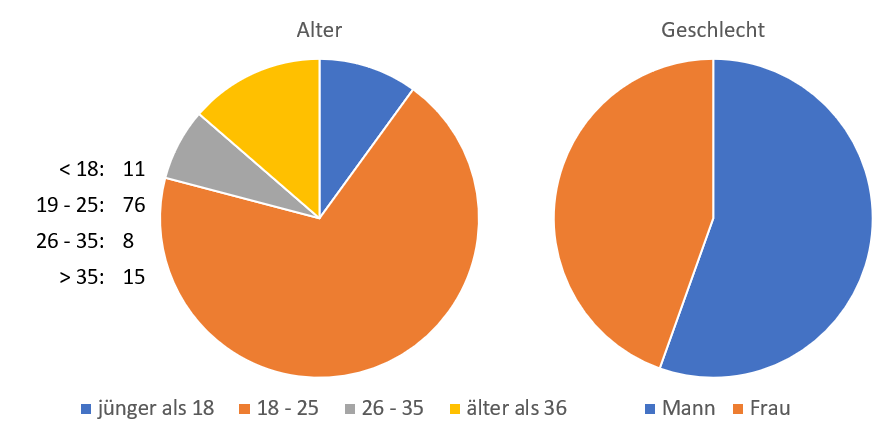
\includegraphics[width=0.7\linewidth]{Picture/umfrage_teilnehmer}
	\caption[Architektur Übersicht]{Architektur Übersicht}
	\label{fig:umfrage_teilnehmer}
\end{figure}

55,5 \% der Teilnehmer sind männlich und 45,5\% sind weiblich. Den Teilnehmern wurden folgende Fragen gestellt:

\begin{enumerate}
	
	\item Wie oft nutzen Sie ein Sprachassistent?
	\item Wissen Sie was mit Ihren Daten passiert?
	\item Würden Sie Geld für eine hohe Datensicherheit bezahlen?
	\item Wie viel Geld würden Sie für eine hohe Datensicherheit einer Anwendung bezahlen (einmalige Zahlung)?
	\item Bei welchen Anwendungen ist Ihnen Privatsphäre besonders wichtig?
	
\end{enumerate}

Bei der ersten Frage stellte sich heraus, dass mehr 54,5\% keine Sprachassistenten verwenden. Die bedeutet, dass 44,5\% einmal in Monat oder häufiger einen solchen Service in Anspruch nehmen. In den USA wurde eine Studie von highervisibility durchgeführt, bei der mehr als 70\% der Teilnehmer einen Sprachassistenten einmal im Monat oder häufiger verwenden\cite{highervisibility}.

\begin{figure}[h!]
	\centering
	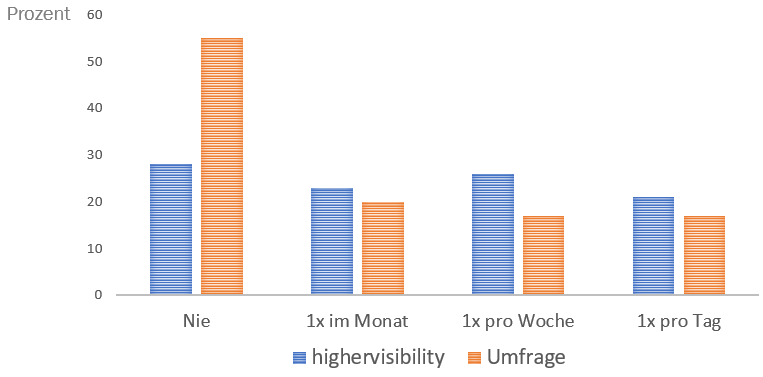
\includegraphics[width=0.7\linewidth]{Picture/umfrage_haeufigkeit}
	\caption[Architektur Übersicht]{Architektur Übersicht}
	\label{fig:umfrage_haeufigkeit}
\end{figure}

Bei den ausgewählten Testpersonen verwenden im Vergleich zur Umfrage, weniger Personen eine Sprachsteuerung. In den USA sind Menschen in verschiedenen Altersgruppe und regionaler Herkunft befragt worden. Die durchgeführte Umfrage hatte überwiegend junge Leute befragt. Erwartet wurde eine höhere Nutzung der Sprachsteuerung. 


Ungefähr 90\% der Teilnehmer haben angegeben, dass sie nicht wissen, was mit ihren Daten passiert. Jeder Vierte würde dabei für eine hohen Datensicherheit Geld bezahlen und 56\% der Teilnehmer sind sich unsicher, ob diese dafür Geld bezahlen würden. Die Altersbetrachtung nach der Zahlungsbereitschaft zeigt, dass die Gruppe unter 18 Jahren weniger bereit ist, Geld zu bezahlen. Die Schnittmenge der Teilnehmern, welche Ja oder vielleicht angekreuzt haben, steigt mit zunehmendem Alter.
\begin{figure}[ht!]
	\centering
	\begin{subfigure}{0.45\linewidth}
		\centering
		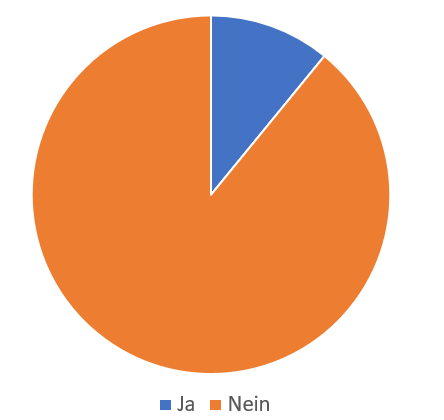
\includegraphics[width=1\linewidth]{Picture/umfrage_datenschutz}
		\caption[Architektur Übersicht]{Architektur Übersicht}
		\label{fig:umfrage_datenschutz}
	\end{subfigure}
	
	\begin{subfigure}{0.45\linewidth}
		\centering
		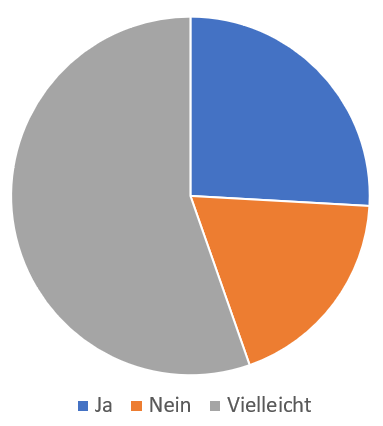
\includegraphics[width=1\linewidth]{Picture/umfrage_geld}
		\caption[Architektur Übersicht]{Architektur Übersicht}
		\label{fig:umfrage_geld}
	\end{subfigure}
	\caption[Architektur Übersicht]{Architektur Übersicht}
	\label{fig:umfrage_datenschutz_geld}
\end{figure}


\begin{figure}[h!]
	\centering
	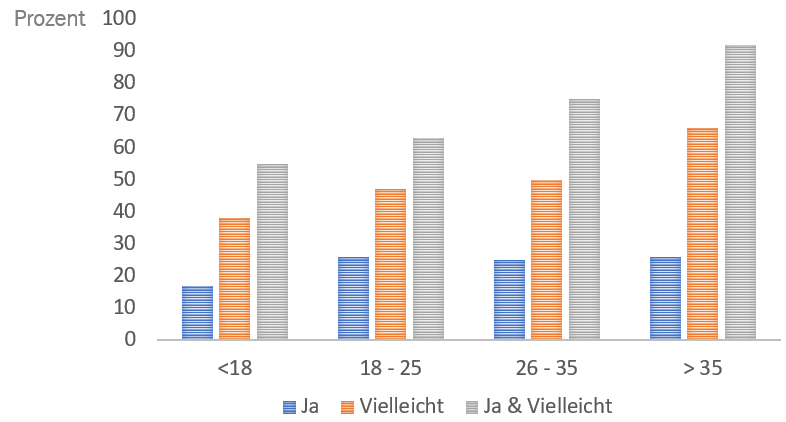
\includegraphics[width=0.7\linewidth]{Picture/umfrage_geld_gruppen}
	\caption[Architektur Übersicht]{Architektur Übersicht}
	\label{fig:umfrage_geld_gruppen}
\end{figure}

Die Beträge welche die Teilnehmer für eine Anwendung bezahlen, bei den ihnen eine hohe Datensicherheit gewährleistet wird, variiert sehr. Hier wären ungefähr 15\% der Teilnehmer nicht bereit für eine bestimmte Anwendung Geld zu zahlen. 85\% sind bereit für eine Anwendung Geld zu bezahlen, bei welcher ihnen ein hoher Datenschutz gewährleistet wird. 

\begin{figure}[h!]
	\centering
	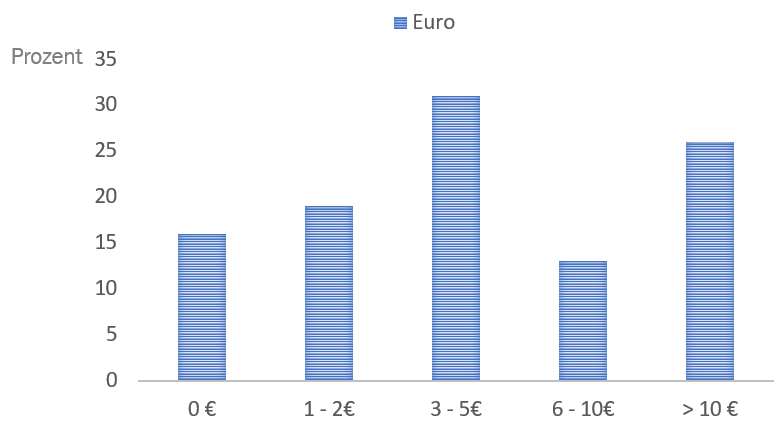
\includegraphics[width=0.7\linewidth]{Picture/umfrage_betrag}
	\caption[Architektur Übersicht]{Architektur Übersicht}
	\label{fig:umfrage_betrag}
\end{figure}

Den Teilnehmern ist die Privatsphäre im Bereich Banking, Haussteuerung, Handysteuerung, Soziale Netzwerke und Chatting besonders wichtig.


\begin{figure}[h!]
	\centering
	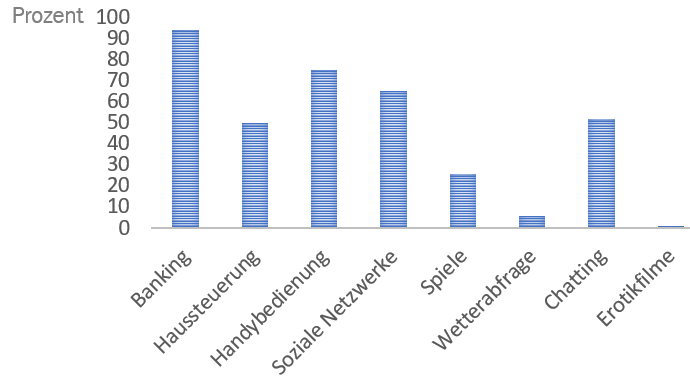
\includegraphics[width=0.7\linewidth]{Picture/umfrage_anwendung}
	\caption[Architektur Übersicht]{Architektur Übersicht}
	\label{fig:umfrage_anwendung}
\end{figure}

Aufgrund dieser Umfrageergebnisse sind wir zu folgenden Schlussfolgerung gekommen:
\begin{itemize}

\item Personen nutzen teilweise Sprachassistenten
\item Die Nutzer wissen nicht, was mit ihren Daten passiert
\item Nutzer würden für bestimmte Anwendungen Geld bezahlen, wenn diese ihre Daten schützt
\item Datenschutz ist in den Bereichen Banking, Chatting, Haussteuerung, Social Media und Handysteuerung wichtig
	
	
\end{itemize}

\subsection{User-Controlled Privacy}

Zu Beginn wird bei dem Konzept darauf verwiesen, dass keine Rahmenbedingungen im Hinblick auf finanzielle Mittel und Rechenressource angenommen sind.
Eine wichtige Anforderung ist der Datenschutz. Die Entwurfsprinzipien für die mehrseitige Sicherheit von Daten stellt folgende vier Punkte in Vordergrund\cite{kairannenberg}:

\begin{itemize}
\item Datensparsamkeit
\item Kontrollmöglichkeiten für den Nutzer 
\item Auswahlmöglichkeiten und Verhandlungsspielräume 
\item Dezentralisierung und Verteilung

\end{itemize}
Der dritte Punkt „Auswahlmöglichkeiten und Verhandlungsspielräume“ sind für dieses Konzept wichtig. Durch eine minimale Datenerfassung wird die Funktionalität von Anwendungen eingeschränkt. Der Benutzer soll darüber entscheiden können, für welche Anwendungen die Funktionalität überwiegen und bei welchen Anwendungen der Datenschutz in Vordergrund steht. Die Punkte Datensparsamkeit, Kontrollmöglichkeiten und Dezentralisierung sollen ebenfalls in den Konzeptentwurf mit einfließen.

Für das oder unser Konzept haben wir folgende Punkte identifiziert, welche beim Entwurf von Sprachassistenten berücksichtigt werden sollten:

\begin{itemize}
\item User-Controlled-Privacy
\item Funktionalität
\item Performance
\item Nutzerfreundlichkeit	
\end{itemize}

Bei der User-Controlled Privacy geht es darum, selbst zu entscheiden, ob der Datenschutz oder die Funktionalität überwiegend im Vordergrund stehen. Funktionalität bedeutet für das Konzept auf eine Funktion verzichten zu müssen, welche andere Anbieter bereitstellen. Die Punkte Performance und Nutzerfreundlichkeit sind eng miteinander verbunden. Bei der Performances geht es darum, eine schnelle Systemantwort zu garantieren, sodass eine solches System der Richtlinien der User Experience entspricht. Die Nutzerfreundlichkeit ist noch weiter gefasst. Nicht nur schnelle Antwortzeiten soll das Konzept garantieren, sondern auch bereitgestellte Konfigurationen, die installiert und gestartet werden können. 

Eine hohe Funktionalität kann durch einen dargestellten Personenkontext berücksichtigt werden, wie in Abbildung ?? zu sehen. Durch dieses Modell können Services auf die unterschiedlichen Nutzerbefindlichkeiten Rücksicht nehmen. In einem Beispielszenario „Hobby Notifier“ kann der Benutzer passende Meldungen erhalten, wenn freie Zeiten in dem Kalender vorhanden sind, das Wetter an dem kommenden Tag gut ist und das Hobby Radfahren sich anbieten würde.



